\def\ktitle{ARM ASSIGNMENT}
\def\kauthor{Koushik Kalyani}
\def\kcontact{koushikkalyani369@gmail.com}
\def\kmodule{IITH - Future Wireless Communication}
\documentclass[journal,12pt,twocolumn]{IEEEtran}
\usepackage{enumitem}
\usepackage{tikz}
\usepackage{circuitikz}
\usepackage{karnaugh-map}
\usepackage{tabularx}
\usepackage{hyperref}
\usepackage{circuitikz}
\usepackage{tikz}
\usepackage{titlesec}
\usepackage{multicol}
\title{\ktitle}
\author{\kauthor\\\kcontact\\\kmodule}
\begin{document}
\maketitle
\tableofcontents
\section{\textbf{Question}}
The logic block shown has an output $F$ given by \rule{12mm}{0.4pt}
\\\resizebox{0.45\textwidth}{!}{
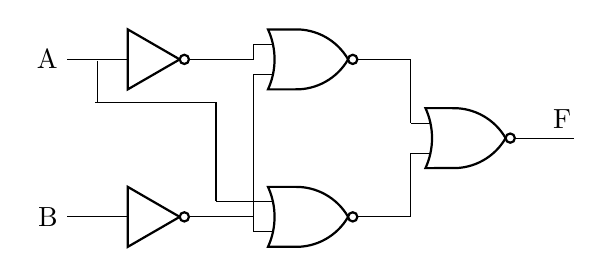
\begin{tikzpicture}
	\ctikzset{
		logic ports=ieee,
		logic ports/scale=0.68,
		logic ports/fill=white}
	\node[not port](x) at (0,0){};
	\node[not port](y) at (0,-2){};
	\node[nor port](a) at (2,0){};
        \node[nor port](b) at (2,-2){};
        \node[nor port](c) at (4,-1){};
	\draw(x.out)-|(a.in 1);
	\draw(y.out)-|(a.in 2);
        \draw(a.out)-|(c.in 1);
        \draw(b.out)-|(c.in 2);
        \draw(0.79,-1.8)|- ++(-1.53,1.25) ;
        \draw(b.in 1)-- ++(-.48,0); 
    %    \draw(-0.72,-2)-- ++(0,-0.55);
      %  \draw(-.72,-2.55)-- ++(1.25,0);
       % \draw(b.in 2)-| ++(-0.72,-.38);
        \draw(-0.72,-.019)-- ++(0,-0.53);
        \draw(y.out)-|(b.in 2);
	\draw(y.in 1)-- ++(-0.5,0) node[left]{B};
        \draw(x.in 1)-- ++(-0.5,0) node[left]{A};
	\draw(c.out)-- ++(0.6,0) node[near end,above]{F};
\end{tikzpicture}
}
\begin{multicols}{2}
\begin{enumerate}[label=(\Alph*)]
	\item $A+B$
	\item $A\cdot \bar B$
	\item $A+ \bar B$
	\item $\bar B$
\end{enumerate}
\end{multicols}
\section{\textbf{Answer}}
The above question can be solved as \\
$\rightarrow \overline{{\overline{\bar A +\bar B} + \overline{A + \bar B}}}$\\
$\rightarrow \overline{A\cdot B + \bar A \cdot B}$\\
$\rightarrow \overline{(A + \bar A ) B}$
$\rightarrow \overline B$\\
Therefore, the output $F=\bar B$. 

\section{\textbf{K-Map Implementation}}
\resizebox{0.45\textwidth}{!}{%
	\begin{karnaugh-map}[2][2][1][B][A]
		\maxterms{1,3}
		\minterms{0,2}
            \implicant{0}{0}
             \implicant{2}{2}
	\end{karnaugh-map}%
}
\centering
Therefore $F=\bar B$
\section{\textbf{Truth Table}}
\begin{tabularx}{0.45\textwidth}{
  | >{\centering\arraybackslash}X  
  | >{\centering\arraybackslash}X 
  | >{\centering\arraybackslash}X |
  }
  \hline
  \textbf{$A$}&\textbf{$B$}&\textbf{$F$}\\
  \hline
  0&0&1\\
  \hline
  0&1&0\\
  \hline
  1&0&1\\
  \hline
  1&1&0\\
  \hline
  \end{tabularx}
\begin{center} 
 Truth table for Boolean funtion $F$
\end{center}
\section{\textbf{Logic Diagram}}
\resizebox{0.45\textwidth}{!}{
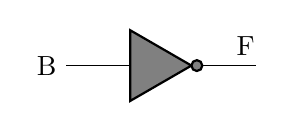
\begin{tikzpicture}
	\ctikzset{
		logic ports=ieee,
		logic ports/scale=0.8,
		logic ports/fill=gray}
	\node[not port](not) at (0,0){};
	
	%\draw(xor.in 1)-- ++(-0.5,0) node[left]{X};
	\draw(not.in)-- ++(-0.5,0) node[left]{B};
	\draw(not.out)-- ++(0.5,0) node[near end,above]{F};
\end{tikzpicture}
}
\begin{center}
	Fig. 2
\end{center}
	\section{\textbf{Components}}
	\begin{tabularx}{0.45\textwidth}{
			| >{\centering\arraybackslash}X
			| >{\centering\arraybackslash}X
			| >{\centering\arraybackslash}X |
			}
			\hline
			\textbf{Components}&\textbf{Values}&\textbf{Quantity}\\
			\hline
			VAMAN & ARM & 1\\
			\hline
			Jumper Wires & F-M & 5\\
			\hline
			Breadboard & & 1\\
			\hline
                LED & & 1\\
                \hline
                Resistor & $\leq 220 \textit{Ohms} $&1\\
                \hline
	\end{tabularx}
\section{\textbf{Implementation}}
\begin{tabularx}{0.45\textwidth}{
		| >{\centering\arraybackslash}X
		| >{\centering\arraybackslash}X
		| >{\centering\arraybackslash}X|}
\hline
	\textbf{VAMAN PIN}&\textbf{INPUT}&\textbf{OUTPUT}\\
	\hline
	22&B& \\
	\hline
	21&&F\\
	\hline

\end{tabularx}\\
\centering
Connections\\
\textbf{Procedure}
\begin{enumerate}[label={\arabic*}.]
	\item Connect the circuit as per the above table.
	\item Connect inputs to Vcc for Logic 1, ground for Logic 0.
	\item Execute the circuit using the below codes.\\
		\vspace{\baselineskip}
		\textit{Approach 1}\\
                \begin{tabularx}{0.45\textwidth}{
				| >{\centering\arraybackslash}X|}
			\hline
         https://github.com/koushikkalyani/FWC/blob\\/main/ARM/main.c \\
			\hline
		\end{tabularx}
		\vspace{\baselineskip}
	\item Change the values of $B$ in the Hardware and verify the Truth Table.
 \end{enumerate}
 \textbf{How to execute}
 \begin{enumerate}[label={\arabic*}.]
     \item Just write your algorithm code in existing code in "main.c".
     \item Go to gcc-project directory and type command "make clean" then to compile type "make".
     \item This will generate .bin file which needs to be sent to your laptop .Connect your mobile Hotspot to your laptop and type command.
     "scp  output/bin/blink.bin pi@192.168.0.114:"change your ip address and in place of pi write your laptop system name.
     \item To see your ip address in your laptop unbuntu terminal connect your hotspot and type "ipconfig".
     \item In your laptop if TinyFPGA is not install then do the following\\
     git clone --recursive https://github.com/QuickLogic-Corp/TinyFPGA-Programmer-Application.git\\
     sudo apt install python3-pip\\
     sudo pip3 install tinyfpgab pyserial\\
     sudo reboot\\
     \item Now download flash.sh and top.bin from the given link\\
     \href{https://github.com/koushikkalyani/FWC/tree/main/ARM}{https://github.com/koushikkalyani/FWC/tree\\/main/ARM}
     \item In flash.sh change directory of tinyfpga according to your system.
     \item flas.sh   top.bin  blink.bin should be in one directory. 
     \item Open terminal and type command "bash flash.sh blink.bin.".
 \end{enumerate}
\end{document}

